\chapter{State of the art}\label{State-of-the-art Methods}
In this section we display some of the most valuable strategies for time series causal discovery, their key concepts, their limitations and their applications, in order to create a solid state of the art set of methods we can use to assess the validity of TD2C (\ref{Experiments}).\\

\section{Granger-Based methods}[\textbf{\textit{Maybe to be reduced}}]\\
Let's start our collection of methods with one of the most pivotal concepts in Causal Inference, the Granger Causality.\\

Based on a statistical version of Hume's regularity theory (Hume, 1738), Granger causality is one of the oldest concepts in causal inference. Hume's theory posits that causal relations can be inferred from the consistent conjunction of causes and effects, with causes preceding their effects. Various authors have investigated probabilistic versions of this theory, which rely on the probability-raising principle (conditioning on a cause increases the probability of the effect occurring). The Granger-based family of methods operates on the premise that if past values of one variable help predict the current value of another, they are causally connected. The simplest implementation, the Pairwise Granger causality test, tests the null hypothesis that $X_i$ does not Granger cause $X_j$ (\textbf{cite TD2C paper}). Granger, in 1969, proposed the following definition:

\begin{definition}
    A time series $X^i$ Granger-causes $X^j$ if past values of $X^i$ provide unique, statistically significant information about future values of $X_j$.
\end{definition}

We could also express it in this way:\\
Let $H_{t-1}$ be the history of all relevant information up to time $t-1$ and $P(X_t | H_{t-1})$ be the optimal prediction of $X_t$ given $H_{t-1}$. Granger defined Y to be causal for X if
$$Var(X_t − P(X_t | H_{t-1}) < Var(X_t − P(X_t | H_{t-1}/F^Y_t)$$
where, $H_{t-1}/F^Y_t$ indicates excluding the values of $F^Y_t$ (Filtration of Y, i.e., all Y values up to time t-1) from $H_{t-1}$ . That is, the variance of the optimal prediction error of X is reduced by including the history of Y (informally, Y is causal of X if past values of Y improve the prediction of X). This characterization is clearly based on predictability
and does not (directly) point to a causal effect of Y on X: Y improving the prediction of X does not mean Y causes X. Nonetheless, assuming causal effects are ordered in time (i.e., cause before effect), Granger argued that, under some assumptions, if Y can predict X, then there must be a mechanistic
(i.e., causal) effect; that is, predictability implies causality. \cite{shojaie2022granger}\\

The concept of Granger Causality has been used in the majority of the exciting causal algorithms today (\cite{guo2020survey}). Despite its widespread use, ongoing debate has surrounded the validity of the Granger causality framework for inferring causal relationships among time series. Additionally, while the original definition was broad, the constraints of computational tools have limited the application of Granger causality mainly to simple bivariate vector autoregressive processes (VAR).(\cite{shojaie2022granger}). Let's dig a bit more into this concepts.\\

Granger causality has traditionally relied on assuming a VAR model and considering tests on its coefficients in the bivariate setting.
Denoting the vector of variables at time $t$ by $X_t = (X^1_t , X^2_t , ..., X^p_t)^T$, we consider the linear model $$A^0X_t = \sum_k = 1^d A^kX_{t−k} + e_t$$ where, $A^0, A^1, ..., A^d$ are $p$ × $p$ lag matrices (coefficients) and $d$, the lag, may be finite or infinite. The term $e_t$, $p$-dimensional white noise innovation, or error, can have a diagonal or non-diagonal covariance matrix $\Sigma$. Granger (1969) highlighted that the model generally lacks identifiability because the matrices $A^k$ are not uniquely defined, except when $A^0$ is diagonal. This special case, which aligns with the well-known VAR model, was specifically noted by Granger (\cite{lutkepohl2005new}) — as a “simple causal model,” opposed to models with instantaneous causal effects whose $A^0$ matrix has nonzero off-diagonal values. This latter form is known as a structural vector autoregressive (SVAR) model (\cite{kilian2013structural}) and can be identified under certain parameter restrictions (\cite{kilian2017structural}).\\

As said, in real-world systems involving multiple time series, examining the relationship between only a pair of series can lead to misleading conclusions due to confounding factors. Specific methods, such as like Network Granger causality, are able address this issue by adjusting for potential confounders and considering multiple series simultaneously. Traditional Granger causal analysis, has also several limitations that restrict its broader application. Specifically, the assumptions required for the (S)VAR model to accurately identify Granger causal relationships include continuous-valued series, linearity, discrete time, known lags, stationarity, perfect observation, and a complete system. Since modern time series data often deviate from these assumptions due to nonlinear dynamics and irregular sampling intervals, recent advancements have made it possible to apply Granger causality to a broader range of scenarios by relaxing these assumptions. \cite{shojaie2022granger}\\

Aside from the most popular GC, there are a few other causality concepts in the field such as Sims Causality, and Intervention Causality. The first one is often treated as a compliment of Granger Causality, where Granger Causality implies Sims Causality but the inverse is not true. Sims stated that a pairwise Granger Causality for $X_t$ and $Y_t$ can be treated as moving average along several lag terms of the two variables, expressed as
$$Y_t = \alpha_1 Y_{t-1} + \beta_1 X_{t-2} + ... + \alpha_k Y_{t-k} + \beta_k+1 X_{t-2} + C + \epsilon$$
where, $k$ represents the combined noise term from both variables. $\alpha$ and $\beta$ terms represent the parameter values at each time lag while $C$ is the combined constant term. Sims Causality stated that variable $X$ does not Granger Cause $Y$ if and only if $\beta_1, \beta_2, ..., \beta_k$ is being chosen identically to zero.

Sims' characterizations, which can be shown to be equivalent to Granger's one, can be tested using an F-test comparing two models: the full model, including past values of both x and y, and the reduced model, including only past values of x. We have $$F = \frac{(RSS_{red} - RSS_{full})/(r-s)}{RSS_{full}/(T-r)}$$
where, $RSS_{full}$ and $RSS_{red}$ are the residual sum of squares for the full and reduced models with $r$ and $s$ parameters, respectively. Using this test, Y is declared Granger causal for X if the observed test statistic $F$ exceeds the (1 − $\alpha$)\% quantile of an $F$-distribution with $r - s$ and $T - r$ degrees of freedom. (\cite{shojaie2022granger})\\

Another causality interpretation, that we call Intervention Causality was proposed by Judea Pearl in 1993 and has been applied to TS data recently. This conception focuses on the idea of counterfactual and calculates the Average Causal Effect (ACE) $$ACE_S = E(Y_{t^*}) - E(Y_t)$$
where, $E(Y_{t^*})$ represents the resulting outcome for variable $Y$ at time $t$ given the occurrence of intervention $S$ and $E(Y_t)$ represents the expected outcome for variable $Y_t$ without the intervention. While concepts such as Granger Causality and Sims Causality assume an observational framework, Intervention Causality requires counterfactual experiments which are not applicable in many real world applications. Our TD2C algorithm falls into the first group. \cite{chang2021multivariate}\\

\section{The 4, 5, 6, ... Families}
In the current literature, there are numerous Causal Discovery methods for both static and time series data. Each method offers unique benefits and faces specific challenges, but the boundaries between them can often be not evident (\cite{hasan2023survey}). Some of these families find application for both types of data, with an obvious more large difficulty for the time-depending ones. In this section we limit our interest in the families whose methods are able to handle successfully this time dependency, and whose application has so far brought at significant results. These methods, as we will see, need to fit in the assumption-wise restricted frame of TD2C method, in order to have a fair and relevant evaluation of this latter.\\
The families we are going to define are the Constraint-based, the Noise-based, the Gradient-based and the Tidybench Methods. The remaining families include all the hybrid methods and other methods that do not fit our main four categories: Score-based (only valid for IID data, i.e., static data), Kernel-based (from which D2C's logic derives it inspiration), Logic-based, Topology-based, Difference-based, ecc. In Figure \ref{fig:2} we summarize schematically what just said.\\

\begin{figure}
    \centering
    \includegraphics[width=1\linewidth]{chapters/Images/Causal Discovery methods.png}
    \caption{Scheme of the most known Causal Discovery methods (in blue, the families we are going to use as benchmarks in the experiments)}
    \label{fig:2}
\end{figure}

\subsection{Contraint-based Methods}\label{Constraint-bsed Methods}
Constraint-based methods in causal discovery rely on graph independencies (\cite{molak2023causal}). A key goal of these methods is testing for conditional independence (CI), which helps recover the causal skeleton when the observed data’s probability distribution is faithful to the underlying causal graph.\cite{runge2020discovering} These approaches aim to determine the presence or absence of edges in the data through the d-separation criterion, i.e. by identifying variables that are d-separated or d-connected. By employing CI tests, constraint-based methods recover the Markov equivalence class of DAGs, assuming faithfulness. Despite their speed, these methods are sensitive to the graph structure and prone to error propagation (\cite{hasan2023survey}).
Some of the most used CB methods are in table \ref{CBm}.

\begin{table}[!ht]
    \centering
    \caption{Table of the most known Constraint-based methods in the literature}
    \begin{tabular}{|l|l|}
    \hline
        \textbf{IID Data} & \textbf{TS Data} \\ \hline
        PC & tsFCI \\ \hline
        FCI & \textcolor{RoyalBlue}{PCMCI} \\ \hline
        ANYTIME FCI & PCMCI+ \\ \hline
        RFCI & LPCMCI \\ \hline
        PC-STABLE & CD-NOD \\ \hline
        PKCL & CDANs \\ \hline
    \end{tabular}
    \label{CBm}
\end{table}

%A problem with large-scale time series data is that although adding more variables makes causal analysis more interpretable, if the additional variables don’t have a significant effect on the causal model, this, in turn, makes the analysis less powerful, and original causal relations may also be overlooked. Moreover, at large dimensions, certain nonlinear tests even lose their ability to limit false positive rates (FPRs). \\

PCMCI is building upon the foundational principles of the PC algorithm. This latter operates operates in three steps: first, identifying the skeleton of the graph by starting with a fully connected undirected graph and then eliminating unconditionally and conditionally independent edges; second, determining V-structures or colliders (e.g., $X \rightarrow Y \leftarrow Z$) using the d-separation set of node pairs; and third, orienting the remaining edges to avoid new V-structures and cycle formation. This process results in a CPDAG, which represents the underlying causal DAG.\\

PCMCI, proposed by Runge et al. (2019), adapts the PC algorithm for time series data, addressing its limitations. It assumes stationarity, causal sufficiency, and the presence of time-lagged dependencies. The algorithm operates in two main stages. In the first stage, it employs PC1, a variant of the skeleton discovery phase of the PC algorithm, to remove irrelevant variables. In the second stage, the algorithm uses the Momentary Conditional Independence (MCI) test to assess whether two variables are independent given their parent sets: $$X^i_{t - \tau} \independent X^j_t | P_A(X^j_t), P_A(X^i_{t - \tau})$$  \cite{hasan2023survey}.

Even when the assumption of stationarity is violated, typically due to obvious confounders, PCMCI still performs more robustly compared to Lasso regression or the PC algorithm. However, PCMCI is less effective for highly predictable systems where little new information is produced at each time step. One significant issue with PCMCI is autocorrelation, which PCMCI+, a more recent version attempts to address. (\cite{runge2020discovering})

\subsection{Gradient-based Methods}
Gradient-based methods stem from research that treats the graph space search as a continuous optimization problem \cite{molak2023causal}. Recent advancements in causal discovery have redefined the structure learning problem as a continuous optimization task, employing a least squares objective alongside an algebraic characterization of Directed Acyclic Graphs (DAGs). This approach transforms the combinatorial structure learning problem into a continuous one, solvable through gradient-based optimization techniques. To further expedite the process, deep learning models capable of capturing intricate nonlinear mappings are often employed. Consequently, these models generally exhibit faster training times, as deep learning is known for its high degree of parallelism on GPUs. They update all edges at each step, considering both the gradient of the score and the acyclicity constraint. \cite{hasan2023survey}\\

\begin{table}[!ht]
    \centering
    \caption{Table of the most known Gradient-based methods in the literature}
    \begin{tabular}{|c|c|c|c|c|}
    \hline
        \textbf{IID Data} & NOTEARS & DAE & GOLEM & MCSL \\ \hline
        \multicolumn{1}{c|}{} & GraN-DAG & DAG-GNN & DAG-NoCurl & ENCO \\ \hline
        \textbf{TS Data} & \textcolor{RoyalBlue}{DYNOTEARS} & NTS-NOTEARS & ~ & ~ \\ \hline
    \end{tabular}
    \label{gbM}
\end{table}

Pamfil et al. (\cite{pamfil2020dynotears}), in 2020, introduced the Dynamic NOTEARS (DYNOTEARS) approach, which is designed for structure learning in dynamic data. DYNOTEARS extends the static NOTEARS method to handle both contemporaneous (intra-slice) and time-lagged (inter-slice) dependencies in dynamic Bayesian networks (DBNs). This methodology involves minimizing a penalized loss function while ensuring that the resulting graph structure is acyclic. The acyclicity constraint is enforced using an algebraic condition that characterizes acyclicity in directed graphs. The method assumes that the structure of the network remains constant over time and is the same across all time series. This fixed-structure assumption simplifies the problem and allows DYNOTEARS to scale effectively to high-dimensional datasets. The approach does not impose implicit constraints on the underlying graph. \cite{hasan2023survey}\\

The model used in DYNOTEARS is a Structural Vector Autoregressive (SVAR) model, where each time series is represented as $X^T_{m,t} = X^T_{m,t}W + X^T_{m,t-1}A_1 + ... + X^T_{m,t-p}A_p + Z^T_{m,t}$ for $t \in {p, ..., T}$ and for all $m \in {1, ..., M}$.. Here, $W$ captures contemporaneous relationships, while $A_1, ..., A_p$ represent time-lagged dependencies. This can be expressed in matrix form as $X = XW + Y_1A_1 + ... + Y_pA_p + Z$, where $X$ is the matrix of observations, $Y$ represents time-lagged versions of $X$, and $Z$ denotes the error terms. The optimization problem tackled by DYNOTEARS involves minimizing the penalized loss function $f(W,A) = \frac{1}{2n}||X - XW - YA||^2_F + \lambda_A||A||_1$ subject to the constraint that $W$ is acyclic. The acyclicity constraint is given by $h(W) = tr(e^{WoW}) - d = 0$, where $o$ denotes the Hadamard product. To solve this optimization problem, DYNOTEARS employs the augmented Lagrangian method, transforming the constrained problem into a series of unconstrained subproblems that can be addressed with standard solvers.\\


\subsection{Noise-based Methods (Functional Methods)}
Drawing inspiration from Independent Component Analysis (ICA), a range of algorithms focuses on unraveling the causal relationships among variables by examining their functional dependencies \cite{molak2023causal}. These algorithms often operate within the framework of Functional Causal Models (FCMs), which articulate the causal connections between variables through specific functional forms. In FCMs, each variable is modeled as a function of its direct causes, accompanied by an independent noise term. This is captured by the equation $$X = f(PA_X) + E$$, where $f$ represents the functional dependency on the parent variables $PA_{X}$, and $E$ denotes the stochastic noise component. By incorporating additional constraints on data distributions or function classes, FCM-based approaches can differentiate between various Directed Acyclic Graphs (DAGs) that belong to the same equivalence class. This capacity to distinguish among DAGs is essential for refining causal inferences and understanding the underlying mechanisms driving the observed data. \cite{hasan2023survey}\\

\begin{table}[!ht]
    \centering
    \caption{Table of the most known Noise-based methods in the literature}
    \begin{tabular}{|c|c|c|c|c|}
    \hline
        \textbf{IID Data} & LiNGAM & ANM & PNL & Direct-LiNGAM \\ \hline
        \multicolumn{1}{c|}{}  & SAM & CGNN & CAM & CAREFL \\ \hline
        \textbf{TS Data} & \textcolor{RoyalBlue}{VarLiNGAM} & TiMINo & ~ & ~ \\ \hline
    \end{tabular}
    \label{nbM}
\end{table}

To uncover the complete causal structure from continuous-valued data, the Linear Non-Gaussian Acyclic Model (LiNGAM) framework is utilized, capitalizing on the independence of non-Gaussian disturbance terms and the linearity of the data-generating process. This approach assumes a recursive causal model, where observed variables are influenced linearly by earlier variables plus non-Gaussian disturbances, without any unobserved confounders (VarLiNGAM also asssumes acyclicity of contemporaneous causal relations). \cite{shimizu2006linear}\\

The core methodology involves Independent Component Analysis (ICA) to identify the underlying causal structure. In a LiNGAM framework, observed data $X$ can be expressed as $X = BX + E$, where $B$ represents the matrix of connection strengths among variables, and $E$ contains the independent, non-Gaussian disturbances. By applying ICA, the model transforms $X = AE$, where $A$ is derived from $(I-B)^{-1}$. ICA's capability to exploit non-Gaussianity allows for a precise estimation of $A$, overcoming the limitations inherent in Gaussian settings where different mixing matrices can yield identical covariance structures. The ICA-based approach does face challenges like the indeterminacies of component order and scaling, but these can be managed by normalizing components and adjusting the matrix $W = A^{-1}$, involved in the 5-steps algorithm. \cite{shimizu2006linear}\\

Building on these principles, the VarLiNGAM algorithm extends the LiNGAM approach by incorporating autoregressive components. This method integrates non-Gaussian instantaneous models with vector autoregressive (VAR) models to estimate both immediate and lagged causal effects. The VarLiNGAM algorithm highlights the importance of accounting for instantaneous influences, as neglecting them can significantly skew the interpretation of time-lagged causal relationships. It demonstrates that, even without prior knowledge of network structure, a non-Gaussian model can be effectively identified, enhancing the accuracy and reliability of causal inference in complex temporal systems. \cite{hasan2023survey}


\subsection{Tidybench Methods (Regression Coefficient-based Methods)}
\textit{\textbf{Evalueate if considering these methods}}\\
- SLARAC, QRBS, LASAR, SELVAR\\

\textit{\textbf{Other eventual Methods relevant for the analysis...}}

\section{D2C \& caD2C}
Finally, we reached the section dedicated to the protagonist of this study, the D2C method. Here we explain its logic and its evolution in the last ten years.\\

\subsection{Introduction to D2C}\label{introd2c}
D2C's main idea has been introduced in 2015 (Bontempi \& Flausder, \cite{bontempi2015dependency}): it's a data driven approach that apply supervised machine learning to infer the causality connections within a multivariate ($n>2$) set of variables. Its main idea relies on the asymmetry generated by two causally related variables that can be noticed in the distribution of their their Markov Blankets' connected variables. It uses some descriptors able to capture this asymmetry and a classifier which learns from artificial data how to discriminate between causal and non causal relations using such descriptors. From its first version (2015), some modifications of the method have been proposed (\cite{bontempi2020learning}, \textbf{\textit{TD2C paper}}) to overcome certain limitations that we will mention later. Anyway, the logic behind the algorithm has remained the same. It is part of the probabilistic methods, (i.e. which infer the probability of existence of a causal link between two variables and then its directionality) relying on observational data, which uses a supervised machine learning approach whose inputs are features able to describe variables' dependency. This ability to reduce uncertainity about the causal relationships using statistical features is common to methods such as ANM (Additive Noise Models), IGCI (Information Geometry Causality Inference), LiNGAM and others. These are able to bypass indistinguishability, which limits the functioning of methods relying on conditional independence (CI) tests, such as Constraint-based approaches. D2C has the merit to expand the field of application of these approaches to multivariate data, a much more complicated operation due to growing parameters and causal interactions.\\
This method is able to derive the relationships between the $n$ variate distribution $X =$ $(X_1,$ $X_2,$ $...,$ $X_n)$ and the existence of a directed causal link between two variables $X_i$ and $X_j$, for $1 \leq i \neq j \leq n$, assuming no confounding, no selection bias and no feedback configurations. 
For the features, it uses structural quantitative characteristics of the data, with the same asymmetry properties, based on information theory concepts (used to quantify the notion of conditional independence), able to derive causality from dependency. Let's see more in detail how the process works in the next section.\\

\subsection{Causality as an asymmetric distribution}
Here we report the mathematical tools that allow us to recognise that asymmetry we mentioned above and to create features able to describe it.\\

First, we need to define dependency
\begin{definition}[Dependency]
    A variable $X_i$ is dependent on a variable $X_j$ if $$p(X_i|X_j = x_j) \neq p(X_i)$$ and we write $X_i \dep X_j$.
\end{definition}
Dependency is symmetric, so, if $X_i \dep X_j \Rightarrow X_j \dep X_i$.\\

Then, we need to define mutual information, and we do it in form of probabilistic density functions:
\begin{equation} \label{eq1}
    I(X_1; X_2) = \int \int log\frac{p(X_1, X_2)}{p(X_1)p)(X_2)}p(X_1, X_2)dX_1dX_2 = H(X_1) - H(X_1|X_2)
\end{equation}
where $H$ is the entropy and we use the convention $0 \ log \ \frac{0}{0}$. This formula measures the amount of stochastic dependence between $X_1$ and $X_2$.\\ 

Dependency becomes, in information terms: $I(X_i; X_j) = I(X_j; X_i) > 0$. It follows that, speaking of conditional mutual information, $I(X_i;X_j|X_z) = 0 \ $ if $ \ p(X_i,X_j|X_z) = p(X_i|X_z)p(X_j|X_z)$, i.e. \textbf{Conditional mutual information between two variables $\bm{X_i}$ and $\bm{X_j}$, given another variable $\bm X_z$, is null if $\bm{X_i}$ and $\bm{X_j}$ are conditionally independent given $\bm{X_z}$, i.e. $\bm X_i \bm\dep \bm X_j \bm| \bm X_z$} (as well as ${I(X_1; X_2) = 0}$ if ${p(X_1, X_2) = p(X_1)p(X_2)}$). The link between this notion and our causality problem is the definition of Markov Blanket:$$I(X_i;(X \symbol{92} (M_i \cup X_i))|M_i) = C_i \cup E_i \cup S_i = 0,$$ where $C_i = {X_c|X_c \rightarrow X_i}$ is the set of variables that have direct arrows pointing to $X_i$ (causes), $E_i = {X_e|X_i \rightarrow X_e}$, are the set of variables to which $X_i$ has a direct causal influence, i.e., where $X_i$ is the parent (effects) and $Si = \{X_s| \ \exists \ X_j : Xs \rightarrow Xj \leftarrow Xi$ and $Xs \neq Xi\}$, are the variables that are not direct causes or effects of $X_i$ but are connected to $X_i$ through a common effect (spouses).\\

Finally, thanks to the \textit{do-operator}, we can define causality, which, instead, is not symmetric in a probabilistic way: We consider, for example, the causal link $X_i \rightarrow X_j$ and we have that $$p(X_j|do(X_i = x_i)) \neq p(X_j), \ but, \ convercely, \ $$  $$p(X_i|do(X_j = x_j)) = p(X_i).$$ Here stands the asymmetry in distribution (Figure \ref{do-}).\\

\

Another way to define causality is graphically, by using a faithful DAG and the rules of d-separation (Figure \ref{fig1}).\\

\begin{figure}[!h]
\centering
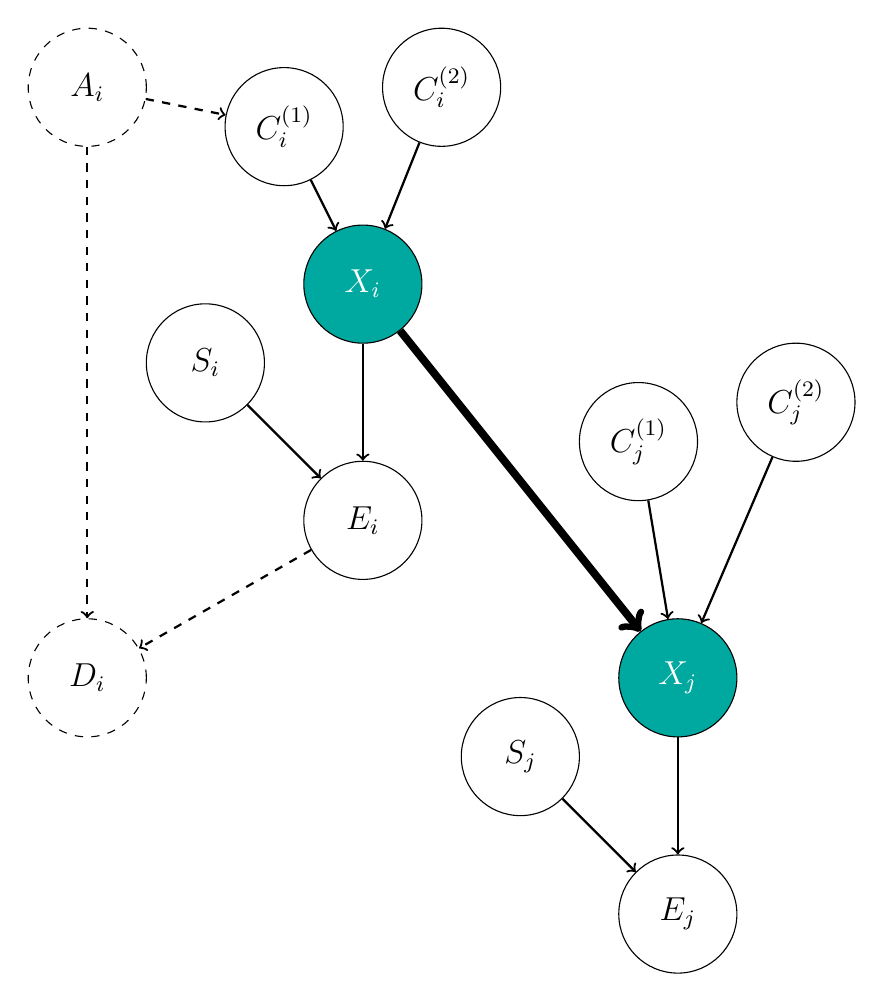
\begin{tikzpicture}[
  every node/.style={draw, circle, minimum size=1.5cm, font=\large},
  dashed node/.style={draw, circle, minimum size=1.5cm, dashed, font=\large},
  dashed edge/.style={draw,->,thick, dashed},
  solid edge/.style={draw,->,thick}
]
% Define the nodes
\node[fill=Emerald, text=white] (A) at (2,2) {$X_i$};
\node[fill=Emerald, text=white] (B) at (6,-3) {$X_j$};
\node (C) at (1,4) {$C^{(1)}_i$};
\node (D) at (2,-1) {$E_i$};
\node (E) at (0,1) {$S_i$};
\node (F) at (5.5,0) {$C^{(1)}_j$};
\node (G) at (6,-6) {$E_j$};
\node (H) at (4,-4) {$S_j$};
\node[dashed node] (I) at (-1.5,4.5) {$A_i$};
\node[dashed node] (J) at (-1.5,-3) {$D_i$};
\node (K) at (3,4.5) {$C^{(2)}_i$};
\node (L) at (7.5,0.5) {$C^{(2)}_j$};
% Define the edges
\path[solid edge, line width=1mm] (A) edge (B);
\path[solid edge] (C) edge (A);
\path[solid edge] (A) edge (D);
\path[solid edge] (E) edge (D);
\path[solid edge] (F) edge (B);
\path[solid edge] (B) edge (G);
\path[solid edge] (H) edge (G);
\path[dashed edge] (I) edge (C);
\path[dashed edge] (D) edge (J);
\path[dashed edge] (I) edge (J);
\path[solid edge] (K) edge (A);
\path[solid edge] (L) edge (B);
\end{tikzpicture}
\caption{ Two causally connected variables ($X_i$ and $X_j$) and their Markov Blankets}
\label{fig1}
\end{figure}

As last, we need to define the descriptors that will be used to train the classifier. We surely need asymmetric measures (not as correlation or mutual information, which are dependency measures, i.e., symmetric: $\rho(i,j) = \rho(j,i)$, $I(i,j) = I(j,i)$). To find such descriptors we rely on the elements in the MBs of the two variables ($M_i, M_j$): $S, C$ and $E$. Thanks to two assumptions: 
\begin{enumerate}
    \item The only path between the sets $X_i \cup M_i$ and $X_j \cup M_j$ is the edge $X_i \rightarrow X_j$.
    \item There are no common ancestors betwween $X_i(X_j)$ and its spouses $S_i(S_j),$
\end{enumerate}
\textbf{\textit{(DOUBT: how to verify these conditions in real-world data)}}

we are able to recognise asymmetric conditional independence relationships between $M_i$ and $M_j$ (Table \ref{table1}(a)), which bring to asymmetric mutual information measures (Table \ref{table2}(a)).\\  

\begin{table}[!ht]
    \centering
    \caption{($\forall k$) All symmetric (b) and asymmetric (a) (un)conditional (in)dependence relationship between $M_i$ and $M_j$ members from \ref{fig1}. Relations $S - C$ and $S - S$ are not considered because they include particular relations, not essential for our goal.}
    \label{table1}
    \begin{tabular}{cc}
        \begin{subtable}[t]{0.45\textwidth}
            \centering
            \caption{ }
            \begin{tabular}{l|l}
            \hline
                \textbf{i - j relations} & \textbf{j - i relations} \\ \hline 
                $X_i \dep C^{k}_j|X_j$ & $X_j \independent C^{k}_i|X_i$ \\ 
                $E_i \dep C^{k}_j|X_j$ & $E_j \independent C^{k}_i|X_i$ \\ 
                $C_i \dep C^{k}_j|X_j$ & $C_j \independent C^{k}_i|X_i$ \\
                $X_i \independent C^{k}_j$ & $X_j \dep C^{k}_i$ \\
                $E_i \independent C^{k}_j$ & $E_j \dep C^{k}_i$ \\ \hline
            \end{tabular}
        \end{subtable} & 
        \begin{subtable}[t]{0.45\textwidth}
            \centering
            \caption{ }
            \begin{tabular}{l|l}
            \hline
                \textbf{i - j relations} & \textbf{j - i relations} \\ \hline
                $X_i \independent E^{k}_j|X_j$ & $X_j \independent E^{k}_i|X_i$ \\ 
                $X_i \independent S^{k}_j|X_j$ & $X_j \independent S^{k}_i|X_i$ \\ 
                $E_i \independent E^{k}_j|X_j$ & $E_j \independent E^{k}_i|X_i$ \\
                $E_i \independent S^{k}_j|X_j$ & $E_j \independent S^{k}_i|X_i$ \\
                $X_i \dep E^{k}_j$ & $X_j \dep E^{k}_i$ \\
                $X_i \independent S^{k}_j$ & $X_j \independent S^{k}_i$ \\
                $E_i \dep E^{k}_j$ & $E_j \dep E^{k}_i$ \\
                $E_i \independent S^{k}_j$ & $E_j \independent S^{k}_i$ \\
                $C_i \independent C^{k}_j$ & $C_j \independent C^{k}_i$ \\ \hline
            \end{tabular}
        \end{subtable} \\
    \end{tabular}
\end{table}

\begin{table}[!ht]
    \centering
    \caption{($\forall k$) All symmetric (b) and asymmetric (a) (un)conditional mutual information between $M_i$ and $M_j$ members from \ref{fig1}. Relations $S - C$ and $S - S$ are not considered because they include particular relations, not essential for our goal.}
    \label{table2}
    \begin{tabular}{cc}
        \begin{subtable}[t]{0.45\textwidth}
            \centering
            \caption{ }
            \begin{tabular}{l|l}
                \hline
                \textbf{i - j relation} & \textbf{j - i relation} \\ \hline
                $I(X_i;C^{k}_j|X_j) > 0$ & $I(X_j; C^{k}_i|X_i) = 0$ \\ 
                $I(E_i;C^{k}_j|X_j) > 0$ & $I(E_j; C^{k}_i|X_i) = 0$ \\ 
                $I(X_i;C^{k}_j|X_j) > 0$ & $I(C_j; C^{k}_i|X_i) = 0$ \\
                $I(C_i; C^{k}_j) = 0$ & $I(X_j \dep C^{k}_i) > 0$ \\
                $I(E_i; C^{k}_j) = 0$ & $I(E_j \dep C^{k}_i) > 0$ \\ \hline
            \end{tabular}
        \end{subtable} & 
        \begin{subtable}[t]{0.45\textwidth}
            \centering
            \caption{ }
            \begin{tabular}{l|l}
                \hline
                \textbf{i - j relation} & \textbf{j - i relation} \\ \hline
                $I(X_i;E^{k}_j|X_j) = 0$ & $I(X_j; E^{k}_i|X_i) = 0$ \\ 
                $I(X_i;S^{k}_j|X_j) = 0$ & $I(Z_j; S^{k}_i|X_i) = 0$ \\ 
                $I(E_i;E^{k}_j|X_j) = 0$ & $I(E_j; E^{k}_i|X_i) = 0$ \\
                $I(E_i;S^{k}_j|X_j) = 0$ & $I(E_j; S^{k}_i|X_i) = 0$ \\
                $I(X_i; S^{k}_j) = 0$ & $I(X_j \dep S^{k}_i) = 0$ \\
                $I(E_i; S^{k}_j) = 0$ & $I(E_j \dep S^{k}_i) = 0$ \\
                $I(C_i; C^{k}_j) = 0$ & $I(C_j \dep C^{k}_i) = 0$ \\
                $I(E_i; E^{k}_j) > 0$ & $I(E_j \dep E^{k}_i) > 0$\\
                $I(X_i; E^{k}_j) > 0$ & $I(X_j \dep E^{k}_i) > 0$ \\
                 \hline
            \end{tabular}
        \end{subtable} \\
    \end{tabular}
\end{table}


The problem is that to know this relationships we need to already know which are the causes, the effects and the spouses in $M_i$ and $M_j$, which is the same information we are trying to derive.\\

To solve this problem, we rely on the following: considering the two MB as mixtures of three distributions (for E, S and C) and knowing that there is an asymmetry within there three described by elements in \ref{table1}(a), even without knowing exactly which role each element assumes (E, S or C), we know the two mixtures are different.\\
Observing the elements in \ref{table2} we notice that, for example, $$
\begin{cases}
    I(X_i;m^{kj}_j|X_j) > I(X_j;m^{ki}_i|X_i) = 0  \ \ \ \ \ \ \ \ if \ \ m^{kj} = C^{kj}_j \ \wedge \  m^{ki} = C^{ki}_i \\
    I(X_i;m^{kj}_j|X_j) = I(X_j;m^{ki}_i|X_i) = 0 \ \ \ \ \ \ \ \ else
\end{cases}
$$
where $m^{ki}$ ($m^{kj}$) is a member of $M_i$ ($M_j$) and we are taking the mixtures of the kind $D_1(i,j) = \{I(X_i; m^{(kj)}_j|X_j)$, $k_j = 1, ..., K_j$\} and $D_1(j,i) = \{I(X_j; m^{(ki)}_i|X_i$), $k_i = 1, ..., K_i$\}. So, as said, the populations $D_1(i,j)$ and $D_1(j,i)$ are different, and we can use them (or some of their moments) as our descriptors of causal dependency. In Table \ref{table3} we put all the asymmetric mixtures D.

\begin{table}[!ht]
    \centering
    \begin{tabular}{l}
    \hline
        \textbf{Asymmetric mixtures} \\ \hline
         (a) $D_1(i,j) = \{I(X_i; m^{(kj)}_j|X_j)$, $k_j = 1, ..., K_j$\}\\
         (b) $D_1(j,i) = \{I(X_j; m^{(ki)}_i|X_i)$, $k_i = 1, ..., K_i$\}\\
         (c) $D_2(i,j) = \{I(m^{(ki)}_i; m^{(kj)_j}|X_j)$, $k_i = 1, ..., K_i$, $k_j = 1, ..., K_j$\}\\
         (d) $D_2(j,i) = \{I(m^{(kj)}_j; m^{(ki)_i}|X_i)$, $k_i = 1, ..., K_i$, $k_j = 1, ..., K_j$\}\\
         (e) $D_3(i,j) = \{I(X_i;m^{(kj)}_j)$, $k_j = 1, ..., K_j$\}\\ (f) $D_3(j,i) = \{I(X_j;m^{(ki)}_i)$, $k_i = 1, ..., K_i$\}
         \\ \hline
    \end{tabular}
    \caption{Asymmetric mixtures from which all the causal descriptors will be generated}
    \label{table3}
\end{table}


\subsection{The algorithm}\label{d2c}
The algorithm starts from two sets of features: one is used to infer the MBs of the two considered variables ($X_i, X_j$) through a filter algorithm (could be mIMR), which also creates a previous relevance ranking within $M_i$ and $M_j$'s elements (we saw that $C$ (causes) elements are much more informative on the direction or causal effects with respect to E (effects) and S (spouses) ones); the other is made by a set of quantiles that summarise the asymmetric mixtures distributions found in the previous section (\ref{table3}). The combined dataset, intended for the classifier, is made of vectors ($d = (d_1, ..., d_i, ..., d_p)$) composed by: a set of mutual information terms between $X_i$ and $X_j$ (estimated as difference of entropy terms, as in \ref{eq1}, through a Lazy Learning algorithm under Gaussian noises assumption), the positions (in the ranking created previously) $P^{ki}_i$ ($P^{kj}_j$) of members $m^{ki}_i$ ($m^{ki}_i$) of $M_i \symbol{92} X_j$ ($M_j \symbol{92} X_i$), the quantiles describing populations in Table \ref{table3} and a binary response variable, \textit{Class}, that indicates the presence (1) or the absence (0) of the causal link. Synthetic dataset of this kind, with complexity $O(Cn + Cn^{'2} + K_iK_jN)$ (\textbf{\textit{specify meanings}}) for each test between two variables, are generated and then used by a Random Forest classifier which, as last step, produces a classification on a testset for validation. In Figure \ref{proc} you can find a graphical representation of the whole process.\\

\textbf{\textit{Insert the formalized algorithm}}.